\section{Introduction}
Definitions are explicit representations of words or phrases that are valuable
for exposing the aspects of a given term. In general, definitions are
unambiguous and succint: they should be easy to read and understand. The
qualities of definitions that allow one to directly understand the meaning of a
word or phrase also allow the exploration of the semantic relationships between
words. These qualities have allowed the creation of neural language models that
can generate useful embeddings based on the semantic information contained in
the definitions \citeauthor{hill_learning_2016, bosc_auto_2018}.

Word embeddings have been taken advantage of in order to obtain powerful
performance in a variety of NLP tasks. They are useful for capturing lexical
syntax and semantics based on word similarity.
\citeauthor{mikolov_distributed_2013} show that basic mathematical operations
applied on word embeddings can show meaningful language understanding
\citeauthor{mikolov_distributed_2013}. However, as continuous representations, the
interpretability of word embeddings is limited.

Thus, the problem of definition modeling was proposed by
\citeauthor{noraset_definition_2016} to evaluate word embeddings
\citeauthor{noraset_definition_2016}. The task of definition modeling is to generate a
definition for a given term. The goal of a model trained on this task is to
train on word embedding and definition pairs in order to learn to generate a
definition for a given word or phrase.

\begin{figure}
    \centering
    

\tikzset{every picture/.style={line width=0.75pt}} %set default line width to 0.75pt        

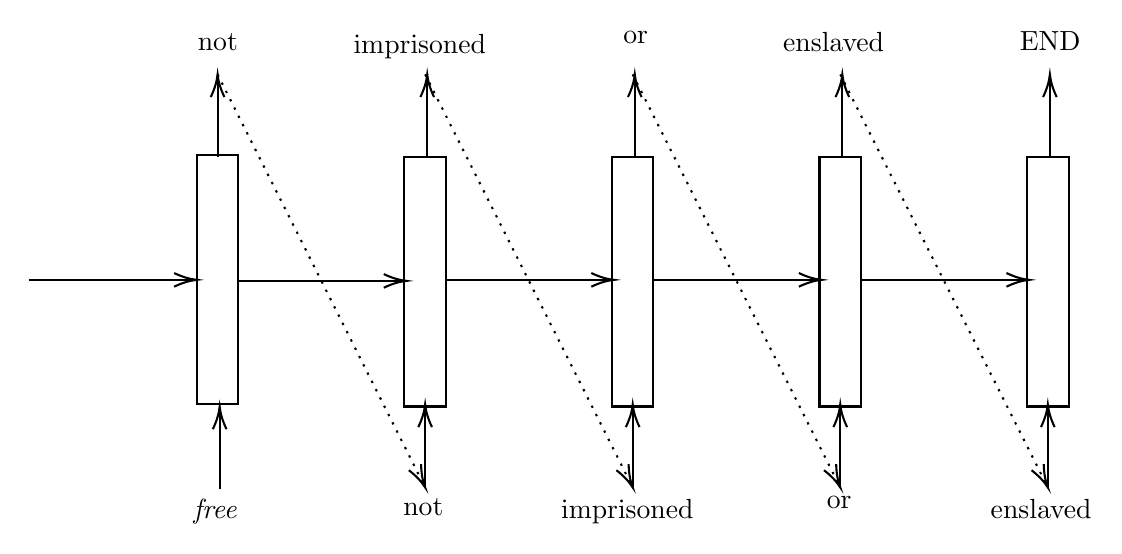
\begin{tikzpicture}[x=0.75pt,y=0.75pt,yscale=-1,xscale=1]
%uncomment if require: \path (0,300); %set diagram left start at 0, and has height of 300

%Straight Lines [id:da39257304513703906] 
\draw    (137,252) -- (137,214) ;
\draw [shift={(137,212)}, rotate = 90] [color={rgb, 255:red, 0; green, 0; blue, 0 }  ][line width=0.75]    (10.93,-3.29) .. controls (6.95,-1.4) and (3.31,-0.3) .. (0,0) .. controls (3.31,0.3) and (6.95,1.4) .. (10.93,3.29)   ;
%Straight Lines [id:da7591784024845039] 
\draw    (236,251) -- (236,213) ;
\draw [shift={(236,211)}, rotate = 90] [color={rgb, 255:red, 0; green, 0; blue, 0 }  ][line width=0.75]    (10.93,-3.29) .. controls (6.95,-1.4) and (3.31,-0.3) .. (0,0) .. controls (3.31,0.3) and (6.95,1.4) .. (10.93,3.29)   ;
%Straight Lines [id:da7914734523205853] 
\draw    (136,92) -- (136,54) ;
\draw [shift={(136,52)}, rotate = 90] [color={rgb, 255:red, 0; green, 0; blue, 0 }  ][line width=0.75]    (10.93,-3.29) .. controls (6.95,-1.4) and (3.31,-0.3) .. (0,0) .. controls (3.31,0.3) and (6.95,1.4) .. (10.93,3.29)   ;
%Straight Lines [id:da4902551924756262] 
\draw    (237,92) -- (237,54) ;
\draw [shift={(237,52)}, rotate = 90] [color={rgb, 255:red, 0; green, 0; blue, 0 }  ][line width=0.75]    (10.93,-3.29) .. controls (6.95,-1.4) and (3.31,-0.3) .. (0,0) .. controls (3.31,0.3) and (6.95,1.4) .. (10.93,3.29)   ;
%Shape: Rectangle [id:dp0975988616572121] 
\draw   (126,91) -- (146,91) -- (146,211) -- (126,211) -- cycle ;
%Shape: Rectangle [id:dp4285052024205802] 
\draw   (226,92) -- (246,92) -- (246,212) -- (226,212) -- cycle ;
%Straight Lines [id:da233208492376886] 
\draw  [dash pattern={on 0.84pt off 2.51pt}]  (136,52) -- (235.1,249.21) ;
\draw [shift={(236,251)}, rotate = 243.32] [color={rgb, 255:red, 0; green, 0; blue, 0 }  ][line width=0.75]    (10.93,-3.29) .. controls (6.95,-1.4) and (3.31,-0.3) .. (0,0) .. controls (3.31,0.3) and (6.95,1.4) .. (10.93,3.29)   ;
%Straight Lines [id:da09388240775198708] 
\draw    (336,251) -- (336,213) ;
\draw [shift={(336,211)}, rotate = 90] [color={rgb, 255:red, 0; green, 0; blue, 0 }  ][line width=0.75]    (10.93,-3.29) .. controls (6.95,-1.4) and (3.31,-0.3) .. (0,0) .. controls (3.31,0.3) and (6.95,1.4) .. (10.93,3.29)   ;
%Straight Lines [id:da30965749620809313] 
\draw    (337,92) -- (337,54) ;
\draw [shift={(337,52)}, rotate = 90] [color={rgb, 255:red, 0; green, 0; blue, 0 }  ][line width=0.75]    (10.93,-3.29) .. controls (6.95,-1.4) and (3.31,-0.3) .. (0,0) .. controls (3.31,0.3) and (6.95,1.4) .. (10.93,3.29)   ;
%Shape: Rectangle [id:dp9002465834996587] 
\draw   (326,92) -- (346,92) -- (346,212) -- (326,212) -- cycle ;
%Straight Lines [id:da04395635540245868] 
\draw  [dash pattern={on 0.84pt off 2.51pt}]  (236,52) -- (335.1,249.21) ;
\draw [shift={(336,251)}, rotate = 243.32] [color={rgb, 255:red, 0; green, 0; blue, 0 }  ][line width=0.75]    (10.93,-3.29) .. controls (6.95,-1.4) and (3.31,-0.3) .. (0,0) .. controls (3.31,0.3) and (6.95,1.4) .. (10.93,3.29)   ;
%Straight Lines [id:da3877015504798327] 
\draw    (436,251) -- (436,213) ;
\draw [shift={(436,211)}, rotate = 90] [color={rgb, 255:red, 0; green, 0; blue, 0 }  ][line width=0.75]    (10.93,-3.29) .. controls (6.95,-1.4) and (3.31,-0.3) .. (0,0) .. controls (3.31,0.3) and (6.95,1.4) .. (10.93,3.29)   ;
%Straight Lines [id:da2270023165703321] 
\draw    (437,92) -- (437,54) ;
\draw [shift={(437,52)}, rotate = 90] [color={rgb, 255:red, 0; green, 0; blue, 0 }  ][line width=0.75]    (10.93,-3.29) .. controls (6.95,-1.4) and (3.31,-0.3) .. (0,0) .. controls (3.31,0.3) and (6.95,1.4) .. (10.93,3.29)   ;
%Shape: Rectangle [id:dp6155481062743988] 
\draw   (426,92) -- (446,92) -- (446,212) -- (426,212) -- cycle ;
%Straight Lines [id:da5303259046258886] 
\draw  [dash pattern={on 0.84pt off 2.51pt}]  (336,52) -- (435.1,249.21) ;
\draw [shift={(436,251)}, rotate = 243.32] [color={rgb, 255:red, 0; green, 0; blue, 0 }  ][line width=0.75]    (10.93,-3.29) .. controls (6.95,-1.4) and (3.31,-0.3) .. (0,0) .. controls (3.31,0.3) and (6.95,1.4) .. (10.93,3.29)   ;
%Straight Lines [id:da8641954739610898] 
\draw    (536,251) -- (536,213) ;
\draw [shift={(536,211)}, rotate = 90] [color={rgb, 255:red, 0; green, 0; blue, 0 }  ][line width=0.75]    (10.93,-3.29) .. controls (6.95,-1.4) and (3.31,-0.3) .. (0,0) .. controls (3.31,0.3) and (6.95,1.4) .. (10.93,3.29)   ;
%Straight Lines [id:da5008199510086007] 
\draw    (537,92) -- (537,54) ;
\draw [shift={(537,52)}, rotate = 90] [color={rgb, 255:red, 0; green, 0; blue, 0 }  ][line width=0.75]    (10.93,-3.29) .. controls (6.95,-1.4) and (3.31,-0.3) .. (0,0) .. controls (3.31,0.3) and (6.95,1.4) .. (10.93,3.29)   ;
%Shape: Rectangle [id:dp9296481241236989] 
\draw   (526,92) -- (546,92) -- (546,212) -- (526,212) -- cycle ;
%Straight Lines [id:da5016591463433577] 
\draw  [dash pattern={on 0.84pt off 2.51pt}]  (436,52) -- (535.1,249.21) ;
\draw [shift={(536,251)}, rotate = 243.32] [color={rgb, 255:red, 0; green, 0; blue, 0 }  ][line width=0.75]    (10.93,-3.29) .. controls (6.95,-1.4) and (3.31,-0.3) .. (0,0) .. controls (3.31,0.3) and (6.95,1.4) .. (10.93,3.29)   ;
%Straight Lines [id:da6856205272297042] 
\draw    (146,151.5) -- (225,151.5) ;
\draw [shift={(227,151.5)}, rotate = 180] [color={rgb, 255:red, 0; green, 0; blue, 0 }  ][line width=0.75]    (10.93,-3.29) .. controls (6.95,-1.4) and (3.31,-0.3) .. (0,0) .. controls (3.31,0.3) and (6.95,1.4) .. (10.93,3.29)   ;
%Straight Lines [id:da08154674166113263] 
\draw    (45,151) -- (93.01,151) -- (124,151) ;
\draw [shift={(126,151)}, rotate = 180] [color={rgb, 255:red, 0; green, 0; blue, 0 }  ][line width=0.75]    (10.93,-3.29) .. controls (6.95,-1.4) and (3.31,-0.3) .. (0,0) .. controls (3.31,0.3) and (6.95,1.4) .. (10.93,3.29)   ;
%Straight Lines [id:da25889258870310994] 
\draw    (246,151) -- (294.01,151) -- (325,151) ;
\draw [shift={(327,151)}, rotate = 180] [color={rgb, 255:red, 0; green, 0; blue, 0 }  ][line width=0.75]    (10.93,-3.29) .. controls (6.95,-1.4) and (3.31,-0.3) .. (0,0) .. controls (3.31,0.3) and (6.95,1.4) .. (10.93,3.29)   ;
%Straight Lines [id:da7935818050042729] 
\draw    (345.99,151) -- (394,151) -- (424.99,151) ;
\draw [shift={(426.99,151)}, rotate = 180] [color={rgb, 255:red, 0; green, 0; blue, 0 }  ][line width=0.75]    (10.93,-3.29) .. controls (6.95,-1.4) and (3.31,-0.3) .. (0,0) .. controls (3.31,0.3) and (6.95,1.4) .. (10.93,3.29)   ;
%Straight Lines [id:da06681494076905437] 
\draw    (446,151) -- (494.01,151) -- (525,151) ;
\draw [shift={(527,151)}, rotate = 180] [color={rgb, 255:red, 0; green, 0; blue, 0 }  ][line width=0.75]    (10.93,-3.29) .. controls (6.95,-1.4) and (3.31,-0.3) .. (0,0) .. controls (3.31,0.3) and (6.95,1.4) .. (10.93,3.29)   ;

% Text Node
\draw (123,255) node [anchor=north west][inner sep=0.75pt]   [align=left] {\textit{free}};
% Text Node
\draw (125,31) node [anchor=north west][inner sep=0.75pt]   [align=left] {not};
% Text Node
\draw (200,31) node [anchor=north west][inner sep=0.75pt]   [align=left] {imprisoned};
% Text Node
\draw (330,30) node [anchor=north west][inner sep=0.75pt]   [align=left] {or};
% Text Node
\draw (407,30) node [anchor=north west][inner sep=0.75pt]   [align=left] {enslaved};
% Text Node
\draw (521,30) node [anchor=north west][inner sep=0.75pt]   [align=left] {END};
% Text Node
\draw (224,255) node [anchor=north west][inner sep=0.75pt]   [align=left] {not};
% Text Node
\draw (300,255) node [anchor=north west][inner sep=0.75pt]   [align=left] {imprisoned};
% Text Node
\draw (428,254) node [anchor=north west][inner sep=0.75pt]   [align=left] {or};
% Text Node
\draw (507,255) node [anchor=north west][inner sep=0.75pt]   [align=left] {enslaved};


\end{tikzpicture}

    \caption{An example of the definition modeling problem for the definiendum
        \textit{free} and an output definition.}
\end{figure}

In addition to being a relatively new language modeling task, definition
modeling has attracted attention from the literature in a number of areas.
First, it was shown that the definition model has poor performance when
generating definitions for polysemes: words with multiple definitions. This
problem was not addressed in the original work as only one definition mapped to
each word. Once researchers attempted to address this problem, they found that
the definition model was unable to learn the semantics of the polyseme with only
the word as an input. Therefore, it was necessary to augment the definition
model with additional information, namely, an example sentence which sets the
word to be defined (\textit{definiendum}) inside to provide context. This method
has been shown to alleviate the problem of generating definitions for polysemes
and also improve the performance of the definition model on several measures
\cite{gadetsky_conditional_2018}, \cite{mickus_mark_2019},
\cite{bevilacqua_generationary_2020}.
